% Copyright (C) 2012 Raniere Silva
% 
% This file is part of 'CNPq 126874/2012-3'.
% 
% 'CNPq 126874/2012-3' is licensed under the Creative Commons
% Attribution 3.0 Unported License. To view a copy of this license,
% visit http://creativecommons.org/licenses/by/3.0/.
% 
% 'CNPq 126874/2012-3' is distributed in the hope that it will be
% useful, but WITHOUT ANY WARRANTY; without even the implied warranty of
% MERCHANTABILITY or FITNESS FOR A PARTICULAR PURPOSE.

\section{Introdução}
Neste trabalho revisitou-se a heurística de reordenamento Cuthill-McKee
Reversa, proposta em 1969, que busca um reordenamento para matrizes esparsas
que reduza a largura de banda destas. O autor deste relatório implementou a heurística
revisitada e utilizou para testar sua implementação problemas da biblioteca
``Netlib LP'' para os quais obteve bons resultados visto que, aproximadamente,
80\% das matrizes testadas tiveram a largura de banda reduzida com o
reordenamento obtido pela heurística e essa redução foi em média de 60\%.

\section{Métodos de Pontos Interiores Primal-Dual}
Consideremos o Problema de Programação Linear na Forma Padrão (PPLFP):
\begin{align*}
    \text{minimizar } & c^T x \\
    \text{sujeito a } & A x = b, \\
    & x \geq 0,
\end{align*}
onde $A \in \mathbb{R}^{m \times n}$ é uma matriz de posto completo $m$ e $c$,
$b$ e $x$ são vetores colunas de dimensão apropriada. Associado a este problema
temos o problema dual (PPLFD):
\begin{align*}
    \text{maximizar } & b^T y \\
    \text{sujeito a } & A^T y + z = c, \\
    & z \geq 0,
\end{align*}
onde $y$ é um vetor coluna de dimensão $m$ de variáveis livres e $z$ é o vetor
coluna de dimensão $n$ de variáveis de folga duais. O \textit{gap} dual é dado
por $\gamma = c^T x - b^T y$ que se reduz a $\gamma = x^T z$ para pontos primais
e duais factíveis.

Os Métodos de Pontos Interiores Primais-Duais para resolver PPLFP consistem em, a
partir de uma tripla inicial $(x^0, y^0, z^0)$, construir uma
sequência de triplas, $(x^i, y^i, z^i)$, dada por
\begin{align*}
    x^{i + 1} &= x^i + \alpha^i \Delta x^i, \\
    y^{i + 1} &= y^i + \alpha^i \Delta y^i, \\
    z^{i + 1} &= z^i + \alpha^i \Delta z^i,
\end{align*}
onde $i \geq 0$ e $\alpha^i \in (0, 1]$, que tende para a tripla $(x^*, y^*, z^*)$ que é
solução de PPLFP e PPLFD. A constante $\alpha^i$ deve ser escolhida tal que $x^i,
z^i > 0$ e, frequentemente, $\alpha^i << 1$ \cite{Wright:1987:PrimalDualIP}.

A direção afim nos Métodos de Pontos Interiores Primais-Duais, $(\Delta x^i,
\Delta y^i, \Delta z^i)$,  é dada por:
\begin{align}
    \begin{bmatrix}
         0 & A^T & I \\
         A & 0 & 0 \\
         Z & 0 & X
     \end{bmatrix} \begin{bmatrix}
         \Delta x^i \\
         \Delta y^i \\
         \Delta z^i
     \end{bmatrix} &= \begin{bmatrix}
         r_d \\
         r_p \\
         r_a
     \end{bmatrix},
     \label{eq:primal_dual_intp:lin_system}
\end{align}
onde $X = \diag(x^i)$, $Z = \diag(z^i)$, $r_p = b - A x^i$, $r_d = c - A^T y^i
- z^i$, $r_a = - X Z e$ e $e$ representa o vetor de uns.

Eliminando as variáveis $\Delta z^i$ de \eqref{eq:primal_dual_intp:lin_system}
obtemos o sistema aumentado:
\begin{align}
    \begin{bmatrix}
        -D & A^T \\
        A & 0
    \end{bmatrix} \begin{bmatrix}
        \Delta x^i \\
        \Delta y^i
    \end{bmatrix} &= \begin{bmatrix}
        r_1 \\
        r_2
    \end{bmatrix},
    \label{eq:primal_dual_intp:aug_lin_system}
\end{align}
onde $D = X^{-1} Z$, $r_1 = r_d - X^{-1} r_a$ e $r_2 = r_p$, e
\begin{align*}
    \Delta z^i &= X^{-1} \left( r_a - Z \Delta x^i \right).
\end{align*}

A forma mais utilizada para resolver \eqref{eq:primal_dual_intp:aug_lin_system}
consiste em reduzir o sistema através de eliminação das variáveis $\Delta x^i$ de
forma a obter o sistema dado por
\begin{align}
    A D^{-1} A^T \Delta y^i &= A D^{-1} r_1 - r_2
    \label{eq:primal_dual_intp:lin_norm}
\end{align}
e que
\begin{align*}
    \Delta x^i &= D^{-1} \left( r_1 - A^T \Delta y^i \right).
\end{align*}

Para resolver \eqref{eq:primal_dual_intp:lin_norm} costuma-se utilizar a
fatoração de Cholesky pois $A D^{-1} A^T$ é uma matriz simétrica definida
positiva. Durante a construção da sequência de triplas $(x^i, y^i, z^i)$ apenas
$D$ muda e por esse motivo a estrutura esparsa de $A D^{-1} A^T$ é mantida
inalterada durante todo o Método de Pontos Interiores Primal-Dual.

\section{Matrizes Esparsas}
Como visto na seção anterior, um dos passos dos Métodos de Pontos Interiores
Primal-Dual consiste em resolver um sistema linear simétrico definido positivo,
cuja estrutura esparsa é mantida inalterada durante todo o método, utilizando a fatoração de
Cholesky. Na próxima subseção introduziremos as definições de banda e envelope
de matrizes para posteriormente apresentarmos a fatoração de Cholesky.

\subsection{Banda e Envelope de Matrizes}
Mudando a notação, considere $A \in \mathbb{R}^{n \times n}$ uma matriz
simétrica definida positiva genérica com entradas $A_{ij}$. Para cada linha $i$
de $A$, $i = 1, \ldots, n$, seja
\begin{align*}
    f_i(A) &= \min\left\{ j \mid A_{ij} \neq 0 \right\},
\end{align*}
isso é, $f_i(A)$ corresponde a primeira coluna cujo elemento na linha $i$ é
diferente de zero.

Seguindo Cuthill e McKee \cite{Cuthill:1969:ReducingBandwidth}, definimos
\begin{align*}
    \beta_i(A) &= i - f_i(A), 1 \leq i \leq n, \\
    \beta(A) &= \max\left\{ \beta_i(A) \mid 1 \leq i \leq n \right\}
\end{align*}
em que $\beta_i(A)$ é a largura de banda da $i$-ésima linha de $A$ e
$\beta(A)$ é a largura de banda da matriz $A$. A banda da matriz $A$ é
definida como
\begin{align*}
    \text{Band}(A) &= \left\{ \left\{ i, j \right\} \mid 0 < i - j \leq
    \beta(A) \right\}
\end{align*}
e ilustrada na Figura~\ref{fig:exem_bandwidth}.
\begin{figure}[!htb]
    \centering
    \begin{tikzpicture}
        \matrix (A) [matrix of math nodes,%
        left delimiter  = \lbrack,%
        right delimiter = \rbrack] at (0,0)
        {%
            1 & 1 & 1 & 1 & 1 & 0 & 0 \\
            1 & 2 & 1 & 1 & 1 & 1 & 1 \\
            1 & 1 & 2 & 1 & 1 & 1 & 1 \\
            1 & 1 & 1 & 2 & 1 & 0 & 0 \\
            1 & 1 & 1 & 1 & 2 & 0 & 0 \\
            0 & 1 & 1 & 0 & 0 & 3 & 2 \\
            0 & 1 & 1 & 0 & 0 & 2 & 3 \\
        };
        \node[above, shift={(0,.5)}] at (A-1-1) {$1$};
        \node[above, shift={(0,.5)}] at (A-1-2) {$2$};
        \node[above, shift={(0,.5)}] at (A-1-3) {$3$};
        \node[above, shift={(0,.5)}] at (A-1-4) {$4$};
        \node[above, shift={(0,.5)}] at (A-1-5) {$5$};
        \node[above, shift={(0,.5)}] at (A-1-6) {$6$};
        \node[above, shift={(0,.5)}] at (A-1-7) {$7$};
        \node[right, shift={(-1.5,0)}] at (A-1-1) {$1$};
        \node[right, shift={(-1.5,0)}] at (A-2-1) {$2$};
        \node[right, shift={(-1.5,0)}] at (A-3-1) {$3$};
        \node[right, shift={(-1.5,0)}] at (A-4-1) {$4$};
        \node[right, shift={(-1.5,0)}] at (A-5-1) {$5$};
        \node[right, shift={(-1.5,0)}] at (A-6-1) {$6$};
        \node[right, shift={(-1.5,0)}] at (A-7-1) {$7$};
        % Largura de banda
        % \draw (A-1-6.north east) -- (A-2-7.north east);
        \draw (A-6-1.south west) -- (A-7-2.south west);
        % Banda
        \fill[gray, fill opacity=0.2, draw=black, dotted] (A-2-1.north west) -- (A-6-1.south west)
        -- (A-6-2.south west) -- (A-7-2.south west) -- (A-7-7.south west)
        \foreach \x in {6,5,4,3,2}{
        -- (A-\x-\x.south east) -- (A-\x-\x.south west) -- (A-\x-\x.north west)
        } -- (A-2-1.north west);

        \matrix (B) [matrix of math nodes,%
        left delimiter  = \lbrack,%
        right delimiter = \rbrack] at (8,0)
        {%
           10 &  0 &  2 &  3 &  0 &  0 &  0 \\
            0 & 10 &  2 &  3 &  0 &  0 &  0 \\
            2 &  2 & 10 &  0 &  4 &  0 &  0 \\
            3 &  3 &  0 & 10 &  4 &  0 &  0 \\
            0 &  0 &  4 &  4 & 10 &  2 &  2 \\
            0 &  0 &  0 &  0 &  2 & 10 &  0 \\
            0 &  0 &  0 &  0 &  2 &  0 & 10 \\
        };
        \node[above, shift={(0,.5)}] at (B-1-1) {$1$};
        \node[above, shift={(0,.5)}] at (B-1-2) {$2$};
        \node[above, shift={(0,.5)}] at (B-1-3) {$3$};
        \node[above, shift={(0,.5)}] at (B-1-4) {$4$};
        \node[above, shift={(0,.5)}] at (B-1-5) {$5$};
        \node[above, shift={(0,.5)}] at (B-1-6) {$6$};
        \node[above, shift={(0,.5)}] at (B-1-7) {$7$};
        \node[right, shift={(-1.5,0)}] at (B-1-1) {$1$};
        \node[right, shift={(-1.5,0)}] at (B-2-1) {$2$};
        \node[right, shift={(-1.5,0)}] at (B-3-1) {$3$};
        \node[right, shift={(-1.5,0)}] at (B-4-1) {$4$};
        \node[right, shift={(-1.5,0)}] at (B-5-1) {$5$};
        \node[right, shift={(-1.5,0)}] at (B-6-1) {$6$};
        \node[right, shift={(-1.5,0)}] at (B-7-1) {$7$};
        % Largura de banda
        % \draw (B-1-4.north east) -- (B-4-7.north east);
        \draw (B-4-1.south west) -- (B-7-4.south west);
        % Banda
        \fill[gray, fill opacity=0.2, draw=black, dotted] (B-1-1.south west) -- (B-4-1.south west)
        -- (B-4-2.south west) -- (B-5-2.south west) -- (B-5-3.south west)
        -- (B-6-3.south west) -- (B-6-4.south west) -- (B-7-4.south west)
        -- (B-7-7.south west)
        \foreach \x in {6,5,4,3,2}{
        -- (B-\x-\x.south east) -- (B-\x-\x.south west) -- (B-\x-\x.north west)
        } -- (B-1-1.south west);
    \end{tikzpicture}
    \caption{Ilustração da banda, sombreado e contornado por pontos, e da
    largura de banda, linha contínua, para duas matrizes simétricas.}
    \label{fig:exem_bandwidth}
\end{figure}

O envelope da matriz $A$ é definido como
\begin{align*}
    \text{Env}(A) &= \left\{ \left\{ i, j \right\} \mid 0 < i - j \leq
    \beta_i(A) \right\}.
\end{align*}
e ilustrado na Figura~\ref{fig:exem_profile}.
\begin{figure}[!htb]
    \centering
    \begin{tikzpicture}
        \matrix (A) [matrix of math nodes,%
        left delimiter  = \lbrack,%
        right delimiter = \lbrack] at (0,0)
        {%
            1 & 1 & 1 & 1 & 1 & 0 & 0 \\
            1 & 2 & 1 & 1 & 1 & 1 & 1 \\
            1 & 1 & 2 & 1 & 1 & 1 & 1 \\
            1 & 1 & 1 & 2 & 1 & 0 & 0 \\
            1 & 1 & 1 & 1 & 2 & 0 & 0 \\
            0 & 1 & 1 & 0 & 0 & 3 & 2 \\
            0 & 1 & 1 & 0 & 0 & 2 & 3 \\
        };
        \node[above, shift={(0,.5)}] at (A-1-1) {$1$};
        \node[above, shift={(0,.5)}] at (A-1-2) {$2$};
        \node[above, shift={(0,.5)}] at (A-1-3) {$3$};
        \node[above, shift={(0,.5)}] at (A-1-4) {$4$};
        \node[above, shift={(0,.5)}] at (A-1-5) {$5$};
        \node[above, shift={(0,.5)}] at (A-1-6) {$6$};
        \node[above, shift={(0,.5)}] at (A-1-7) {$7$};
        \node[right, shift={(-1.5,0)}] at (A-1-1) {$1$};
        \node[right, shift={(-1.5,0)}] at (A-2-1) {$2$};
        \node[right, shift={(-1.5,0)}] at (A-3-1) {$3$};
        \node[right, shift={(-1.5,0)}] at (A-4-1) {$4$};
        \node[right, shift={(-1.5,0)}] at (A-5-1) {$5$};
        \node[right, shift={(-1.5,0)}] at (A-6-1) {$6$};
        \node[right, shift={(-1.5,0)}] at (A-7-1) {$7$};
        % Perfil
        \fill[gray, fill opacity=0.2, draw=black, dotted] (A-2-1.north west) -- (A-6-1.north
        west) -- (A-6-2.north west) --
        (A-7-2.south west) -- (A-7-7.south west)
        \foreach \x in {6,5,4,3,2}{
        -- (A-\x-\x.south east) -- (A-\x-\x.south west) -- (A-\x-\x.north west)
        } -- (A-2-1.north west);

        \matrix (B) [matrix of math nodes,%
        left delimiter  = \lbrack,%
        right delimiter = \rbrack] at (8,0)
        {%
           10 &  0 &  2 &  3 &  0 &  0 &  0 \\
            0 & 10 &  2 &  3 &  0 &  0 &  0 \\
            2 &  2 & 10 &  0 &  4 &  0 &  0 \\
            3 &  3 &  0 & 10 &  4 &  0 &  0 \\
            0 &  0 &  4 &  4 & 10 &  2 &  2 \\
            0 &  0 &  0 &  0 &  2 & 10 &  0 \\
            0 &  0 &  0 &  0 &  2 &  0 & 10 \\
        };
        \node[above, shift={(0,.5)}] at (B-1-1) {$1$};
        \node[above, shift={(0,.5)}] at (B-1-2) {$2$};
        \node[above, shift={(0,.5)}] at (B-1-3) {$3$};
        \node[above, shift={(0,.5)}] at (B-1-4) {$4$};
        \node[above, shift={(0,.5)}] at (B-1-5) {$5$};
        \node[above, shift={(0,.5)}] at (B-1-6) {$6$};
        \node[above, shift={(0,.5)}] at (B-1-7) {$7$};
        \node[right, shift={(-1.5,0)}] at (B-1-1) {$1$};
        \node[right, shift={(-1.5,0)}] at (B-2-1) {$2$};
        \node[right, shift={(-1.5,0)}] at (B-3-1) {$3$};
        \node[right, shift={(-1.5,0)}] at (B-4-1) {$4$};
        \node[right, shift={(-1.5,0)}] at (B-5-1) {$5$};
        \node[right, shift={(-1.5,0)}] at (B-6-1) {$6$};
        \node[right, shift={(-1.5,0)}] at (B-7-1) {$7$};
        % Perfil
        \fill[gray, fill opacity=0.2, draw=black, dotted] (B-2-1.south west) -- (B-5-1.north
        west) -- (B-5-3.north west) --
        (B-5-3.south west) -- (B-6-5.north west) -- (B-7-5.south west)
        -- (B-7-7.south west)
        \foreach \x in {6,5,4,3}{
        -- (B-\x-\x.south east) -- (B-\x-\x.south west) -- (B-\x-\x.north west)
        } -- (B-2-1.south west);
    \end{tikzpicture}
    \caption{Ilustração do envelope, sombreado e contornado por
    pontos, para duas matrizes simétricas.}
    \label{fig:exem_profile}
\end{figure}

\subsection{Fatoração de Cholesky}
Seja $A \in \mathbb{R}^{n \times n}$ uma matriz simétrica definida positiva, então existe
uma única matriz $G \in \mathbb{R}^{n \times n}$ triangular inferior com
elementos positivos na diagonal tal que $A = G G^T$. A fatoração $A = G G^T$ é
conhecida como fatoração de Cholesky e no algoritmo a seguir é apresentado
uma forma de obter-se $G$.
\begin{algorithm}[hbt]
    \caption{Pseudo-código da Fatoração de Cholesky}
    \label{alg:chol}
    \begin{algorithmic}[1]
        \REQUIRE $A \in \mathbb{R}^{n \times n}$ simétrica definida positiva.
        \ENSURE $G \in \mathbb{R}^{n \times n}$
        \STATE $G \longleftarrow 0$ 
        \FOR{$k \in 1, \ldots, n$}
            \STATE $G_{k,k} \longleftarrow \sqrt{A_{k,k}}$ \label{alg:chol:sqrt}
            \FOR{$i \in k+1, \ldots n$}
                \STATE $G_{i,k} \longleftarrow A_{i,k} / G_{k,k}$
                \label{alg:chol:div}
            \ENDFOR
            \FOR{$j \in k+1, \ldots, n$}
                \FOR{$i \in k+1, \ldots, n$}
                    \STATE $A_{i,j} \longleftarrow A_{i,j} - G_{i,k} G_{j,k}$
                    \label{alg:chol:prod}
                \ENDFOR
            \ENDFOR
        \ENDFOR
    \end{algorithmic}
\end{algorithm}

\begin{prop}
    \label{prop:pres:env}
    A fatoração de Cholesky preserva o envelope da matriz.
\end{prop}
\begin{proof}
    Para calcular $G$ no Algoritmo~\ref{alg:chol} ocorrem operações aritméticas
    apenas nas linhas \ref{alg:chol:sqrt}, \ref{alg:chol:div} e
    \ref{alg:chol:prod}. Vamos mostrar que nenhuma dessas operações aritméticas
    altera o envelope da matriz.

    Para a linha \ref{alg:chol:sqrt}, como $A$ é simétrica definida positiva,
    ocorre que $A_{k,k}$ é não nulo e, portanto, $G_{k,k}$ também.

    Para a linha \ref{alg:chol:div} é fácil verificar que $G_{i,k}$ é nulo se e
    somente se $A_{i,k}$.

    Para a linha \ref{alg:chol:prod}, se $A_{i,j}$ não pertence ao envelope de $A$
    então $A_{i,j}$ e $G_{i,k}$ são nulos e portanto o envelope não é alterado.
\end{proof}

\begin{prop}
    \label{prop:pres:band}
    A fatoração de Cholesky preserva a banda da matriz.
\end{prop}
\begin{proof}
    Como o envelope da matriz está contido na banda da matriz e já provamos que
    a fatoração de Cholesky preserva o envelope podemos concluir que a fatoração
    de Cholesky também preserva a banda da matriz.
\end{proof}

\section{Cuthill-McKee reverso}
Considere a matriz $A$ e seu fator de Cholesky $G$ dados por
\begin{align*}
    A &= \begin{bmatrix}
        1 &  1 &  1 &  1 &  1 &  1 &  1 \\
        1 & 10 &  0 &  0 &  0 &  0 &  0 \\
        1 &  0 & 10 &  0 &  0 &  0 &  0 \\
        1 &  0 &  0 & 10 &  0 &  0 &  0 \\
        1 &  0 &  0 &  0 & 10 &  0 &  0 \\
        1 &  0 &  0 &  0 &  0 & 10 &  0 \\
        1 &  0 &  0 &  0 &  0 &  0 & 10
    \end{bmatrix}, & G &= \begin{bmatrix}
        1.0 &  0.0 &  0.0 &  0.0 &  0.0 &  0.0 &  0.0 \\
        1.0 &  3.0 &  0.0 &  0.0 &  0.0 &  0.0 &  0.0 \\
        1.0 & -0.3 &  2.9 &  0.0 &  0.0 &  0.0 &  0.0 \\
        1.0 & -0.3 & -0.3 &  2.9 &  0.0 &  0.0 &  0.0 \\
        1.0 & -0.3 & -0.3 & -0.4 &  2.9 &  0.0 &  0.0 \\
        1.0 & -0.3 & -0.3 & -0.4 & -0.4 &  2.8 &  0.0 \\
        1.0 & -0.3 & -0.3 & -0.4 & -0.4 & -0.5 &  2.8
    \end{bmatrix}.
\end{align*}
Observa-se que vários elementos nulos na parte triangular inferior de $A$ são
não nulos em $G$. A perda de elementos nulos ao realizar a fatoração de
Cholesky é denominada de preenchimento e deve ser evitada sempre que possível.

Na seção anterior verificou-se que a fatoração de Cholesky preserva a banda e
envelope da matriz. Por esse motivo, ao utilizar matrizes de banda e
envelope pequenos o preenchimento da matriz também será pequeno. Será que dada
uma matriz $A \in \mathbb{R}^{n \times n}$ simétrica definida positiva existe
uma matriz $A' = P A P^T$, onde $P$ é uma matriz de permutação, tal que a banda
e/ou envelope de $A'$ é menor que o de $A$?

\begin{exem}
    Considere a matriz $A$ e $G$ dada por
    \begin{align*}
        A &= \begin{bmatrix}
            1 & 1 & 1 & 1 & 1 & 0 & 0 \\
            1 & 2 & 1 & 1 & 1 & 1 & 1 \\
            1 & 1 & 2 & 1 & 1 & 1 & 1 \\
            1 & 1 & 1 & 2 & 1 & 0 & 0 \\
            1 & 1 & 1 & 1 & 2 & 0 & 0 \\
            0 & 1 & 1 & 0 & 0 & 3 & 2 \\
            0 & 1 & 1 & 0 & 0 & 2 & 3
        \end{bmatrix},
        & G &= \begin{bmatrix}
            1 & 0 & 0 & 0 & 0 & 0 & 0 \\
            1 & 1 & 0 & 0 & 0 & 0 & 0 \\
            1 & 0 & 1 & 0 & 0 & 0 & 0 \\
            1 & 0 & 0 & 1 & 0 & 0 & 0 \\
            1 & 0 & 0 & 0 & 1 & 0 & 0 \\
            0 & 1 & 1 & 0 & 0 & 1 & 0 \\
            0 & 1 & 1 & 0 & 0 & 0 & 1
        \end{bmatrix}.
    \end{align*}
    Verifica-se que a largura da banda de $A$ e $G$ é $5$ e o envelope é $19$.

    Agora, considere a matriz $A' = P A P^T = G' G'^T$, em que $P$ é uma matriz de
    permutação, dada por
    % O vetor de permutação é
    % [4, 3, 0, 2, 1, 6, 5]
    \begin{align*}
        A' &= \begin{bmatrix}
            2 & 1 & 1 & 1 & 1 & 0 & 0 \\
            1 & 2 & 1 & 1 & 1 & 0 & 0 \\
            1 & 1 & 1 & 1 & 1 & 0 & 0 \\
            1 & 1 & 1 & 2 & 1 & 1 & 1 \\
            1 & 1 & 1 & 1 & 2 & 1 & 1 \\
            0 & 0 & 0 & 1 & 1 & 3 & 2 \\
            0 & 0 & 0 & 1 & 1 & 2 & 3
        \end{bmatrix},
        & G' &= \begin{bmatrix}
             1.4 & 0 & 0 & 0 & 0 & 0 & 0 \\
            0.70 & 1.2 & 0 & 0 & 0 & 0 & 0 \\
            0.70 & 0.40 & 0.57 & 0 & 0 & 0 & 0 \\
            0.70 & 0.40 & 0.57 & 1 & 0 & 0 & 0 \\
            0.70 & 0.40 & 0.57 & 0 & 1 & 0 & 0 \\
            0 & 0 & 0 & 1 & 1 & 1 & 0 \\
            0 & 0 & 0 & 1 & 1 & 0 & 1
        \end{bmatrix}
    \end{align*}
    Verifica-se que a largura da banda de $A$ e $G$ é $4$ e o envelope é $15$.
\end{exem}

Pelo exemplo anterior, verifica-se a possibilidade de preprocessar a matriz
de forma a reduzir a banda e envelope.

Na próxima subseção apresentamos algumas definições da Teoria de Grafos que
serão utilizadas no algoritmo estudado para obter uma permutação que busca
reduzir a largura de banda e envelope.

\subsection{Grafos e matrizes esparsas}
Um grafo é, fundamentalmente, um modo de representar uma relação binária entre
objetos. Para o propósito deste trabalho, considere um grafo $G = (V, E)$ como
um conjunto de vértices $V = \{v_1, v_2, \ldots \}$ e um conjunto de
arestas $E = \{e_1, e_2, \ldots \}$, que são representadas por pares
não ordenados, por exemplo, $e_1 = \{v_1 , v_2\}$.

Assim como um grafo, uma matriz também descreve uma relação binária entre objetos
através de seus elementos não nulos. Uma matriz simétrica $A \in \mathbb{R}^{n
\times n}$ induz um grafo $G(A)$, onde os vértices do grafo correspondem as
dimensões da matriz e a aresta $e = \{i, j\}$ existe se e somente se $A_{ij} \neq 0$.
Na figura abaixo é ilustrado a relação entre uma matriz e um grafo.
\begin{figure}[!hbt]
    \centering
    \begin{tikzpicture}
        \matrix (A) [matrix of math nodes,%
        left delimiter  = \lbrack,%
        right delimiter = \rbrack] at (0,0)
        {%
            1 & 1 & 1 & 1 & 1 & 0 & 0 \\
            1 & 2 & 1 & 1 & 1 & 1 & 1 \\
            1 & 1 & 2 & 1 & 1 & 1 & 1 \\
            1 & 1 & 1 & 2 & 1 & 0 & 0 \\
            1 & 1 & 1 & 1 & 2 & 0 & 0 \\
            0 & 1 & 1 & 0 & 0 & 3 & 2 \\
            0 & 1 & 1 & 0 & 0 & 2 & 3 \\
        };
        %Graph
        \node[draw, circle] (1) at (6,0) {1};
        \node[draw, circle] (2) at (8,1) {2};
        \node[draw, circle] (3) at (8,-1) {3};
        \node[draw, circle] (4) at (4,1) {4};
        \node[draw, circle] (5) at (4,-1) {5};
        \node[draw, circle] (6) at (10,1) {6};
        \node[draw, circle] (7) at (10,-1) {7};
        \draw (1) -- (2);
        \draw (1) -- (3);
        \draw (1) -- (4);
        \draw (1) -- (5);
        \draw (2) -- (3);
        \draw (2) -- (4);
        \draw (2) to[out=190, in=60] (5);
        \draw (2) -- (6);
        \draw (2) -- (7);
        \draw (3) to[out=120, in=-10] (4);
        \draw (3) -- (5);
        \draw (3) -- (6);
        \draw (3) -- (7);
        \draw (4) -- (5);
        \draw (6) -- (7);
    \end{tikzpicture}
    \caption{Ilustração do grafo (a direita) correspondente a uma matriz (a
    esquerda).}
    \label{fig:exem_matrix2graph}
\end{figure}

É importante destacar que permutar, simetricamente, linhas e colunas de uma
matriz corresponde a renumerar os vértices do grafo. Na
Figura~\ref{fig:exem_matrix2graph_perm} é ilustrado uma permutação da matriz
presente na Figura~\ref{fig:exem_matrix2graph} e a renumeração dos vértices do
grafo.
\begin{figure}[!hbt]
    \centering
    \begin{tikzpicture}
        \matrix (A) [matrix of math nodes,%
        left delimiter  = \lbrack,%
        right delimiter = \rbrack] at (0,0)
        {%
            2 & 1 & 1 & 1 & 1 & 0 & 0 \\
            1 & 2 & 1 & 1 & 1 & 0 & 0 \\
            1 & 1 & 1 & 1 & 1 & 0 & 0 \\
            1 & 1 & 1 & 2 & 1 & 1 & 1 \\
            1 & 1 & 1 & 1 & 2 & 1 & 1 \\
            0 & 0 & 0 & 1 & 1 & 3 & 2 \\
            0 & 0 & 0 & 1 & 1 & 2 & 3 \\
        };
        %Graph
        \node[draw, circle] (1) at (6,0) {3};
        \node[draw, circle] (2) at (8,1) {4};
        \node[draw, circle] (3) at (8,-1) {5};
        \node[draw, circle] (4) at (4,1) {2};
        \node[draw, circle] (5) at (4,-1) {3};
        \node[draw, circle] (6) at (10,1) {6};
        \node[draw, circle] (7) at (10,-1) {7};
        \draw (1) -- (2);
        \draw (1) -- (3);
        \draw (1) -- (4);
        \draw (1) -- (5);
        \draw (2) -- (3);
        \draw (2) -- (4);
        \draw (2) to[out=190, in=60] (5);
        \draw (2) -- (6);
        \draw (2) -- (7);
        \draw (3) to[out=120, in=-10] (4);
        \draw (3) -- (5);
        \draw (3) -- (6);
        \draw (3) -- (7);
        \draw (4) -- (5);
        \draw (6) -- (7);
    \end{tikzpicture}
    \caption{Ilustração da permutação simétrica de uma matriz e a renumeração
    dos vértices do grafo correspondente.}
    \label{fig:exem_matrix2graph_perm}
\end{figure}

Um resumo dos principais conceitos é dado a seguir:
\begin{description}
    \item[Vértices adjacentes]  dois vértices $v_1$ e $v_2$ são adjacentes
        quando existe uma aresta entre eles, ou seja, $\{v_1, v_2\} \in E$.
    \item[Incidência] uma aresta incide em um vértice se ele for um dos extremos
        da aresta.
    \item[Grau do vértice] número de arestas incidentes no vértice.
    \item[Caminho] sequência de arestas disjuntas $\left( (x_1, x_2), (x_2,
        x_3), \ldots (x_{k - 1}, x_k) \right)$. O tamanho de um caminho é o
        número de arestas que o compõe.
    \item[Grafo conectado (conexo)] possui pelo menos um caminho entre qualquer
        par de vértices.
    \item[Distância entre vértices] ou $d(v_1, v_2)$, número de arestas que
        formam o menor caminho ligando os vértices $v_1$ e $v_2$.
    \item[Excentricidade] ou $l(v)$, maior distância do vértice $v$ a qualquer outro.
    \item[Diâmetro] maior excentricidade dentre os vértices de um grafo.
    \item[Pseudo-diâmetro] corresponde a uma alta excentricidade, porém não
        necessariamente a maior de todas.
    \item[Vértices periféricos] são vértices cuja excentricidade é igual ao
        diâmetro do grafo.
    \item[Vértices pseudo-periféricos] são vértices que apresentam altas
        excentricidades, mas não necessariamente a maior.
    \item[Estrutura de nível] é uma partição do conjunto $V$ em níveis $L_0,
        L_2, \ldots, L_{l(v)}$ tal que
        \begin{enumerate}
            \item todos os vértices adjacentes aos vértices do nível $L_0$
                encontram-se nos níveis $L_0$ ou $L_1$,
            \item todos os vértices adjacentes aos vértices no nível $L_{l(v)}$
                encontram-se nos níveis $L_{l(v)}$ ou $L_{l(v) - 1}$,
            \item para $0 < i < l(v)$, todos os vértices no nível $L_i$
                encontram-se nos níveis $L_{i - 1}$, $L_i$ ou $L_{i + 1}$.
        \end{enumerate}

        A estrutura de nível com raiz no vértice $v$ é corresponde a
        \begin{enumerate}
            \item $L_0 = \left\{ v \right\}$,
            \item para $i > 0$, $L_i$ é o conjunto de vértices adjacentes aos
                vértices presentes no nível $L_{i - 1}$ e ainda não pertencentes
                a nenhum nível.
        \end{enumerate}

        Na Figura~\ref{fig:graph2level_struct} é ilustrado a estrutura de
        nível, dentre as várias possíveis, para um grafo.
\end{description}
\begin{figure}[htb]
    \centering
    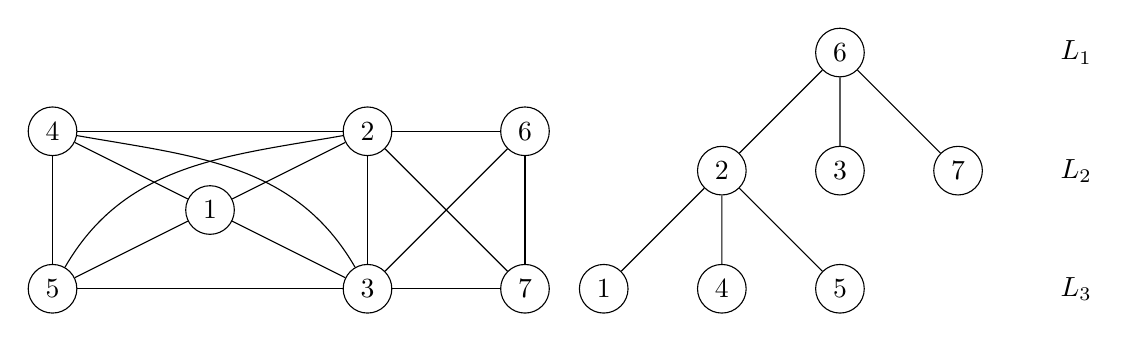
\begin{tikzpicture}
        % graph
        \node[draw, circle] (1) at (2,0) {1};
        \node[draw, circle] (2) at (4,1) {2};
        \node[draw, circle] (3) at (4,-1) {3};
        \node[draw, circle] (4) at (0,1) {4};
        \node[draw, circle] (5) at (0,-1) {5};
        \node[draw, circle] (6) at (6,1) {6};
        \node[draw, circle] (7) at (6,-1) {7};
        \draw (1) -- (2);
        \draw (1) -- (3);
        \draw (1) -- (4);
        \draw (1) -- (5);
        \draw (2) -- (3);
        \draw (2) -- (4);
        \draw (2) to[out=190, in=60] (5);
        \draw (2) -- (6);
        \draw (2) -- (7);
        \draw (3) to[out=120, in=-10] (4);
        \draw (3) -- (5);
        \draw (3) -- (6);
        \draw (3) -- (7);
        \draw (4) -- (5);
        \draw (6) -- (7);
        % level structure
        \node[draw, circle] at (10,2) {6}
            child { node[draw, circle] {2}
                child { node[draw, circle] {1} }
                child { node[draw, circle] {4} }
                child { node[draw, circle] {5} } } 
            child { node[draw, circle] {3} }
            child { node[draw, circle] {7} };
        \path[white, text=black] node at (13,2) {$L_1$}
            child { node {$L_2$}
                child { node {$L_3$} } };
    \end{tikzpicture}
    \caption{Grafo (esquerda) e sua estrutura de nível com raiz no vértice 6
    (direita).}
    \label{fig:graph2level_struct}
\end{figure}
\subsection{Método Cuthill-McKee Reverso}
Cuthill e McKee \cite{Cuthill:1969:ReducingBandwidth} propuseram uma heurística de
reordenação, ver algoritmo abaixo, cujo objetivo principal é reduzir a largura
de banda de uma matriz simétrica $A \in \mathbb{R}^{n \times n}$ cujo grafo
é conexo.
\begin{algorithm}[hbt]
    \caption{Pseudo-código de Cuthill-McKee}
    \label{alg:rcm}
    \begin{algorithmic}[1]
        \REQUIRE Grafo $G(A)$ e um vértice inicial $v$.
        \ENSURE $o$, novo ordenamento dos vértices de $G(A)$.
        \STATE Marca todos os vértices como não visitados.
        \STATE $o \longleftarrow \text{ vetor de zeros}$
        \STATE $i \longleftarrow 1$
        \STATE $f \longleftarrow \text{ fila vazia}$
        \STATE Adicionar $v$ na fila $f$.
        \STATE Marca $v$ como visitado.
        \WHILE{$f$ não for vazia}
            \STATE Desenfileira $f$ em $v$.
            \STATE $o_i \longleftarrow v$
            \STATE $i \longleftarrow i + 1$
            \FORALL{vértice $w$ adjacente a $v$, em ordem crescente de grau,}
                \IF{$w$ ainda não foi visitado}
                    \STATE Adicionar $v$ na fila $f$.
                    \STATE Marca $w$ como visitado.
                \ENDIF
            \ENDFOR
        \ENDWHILE
    \end{algorithmic}
\end{algorithm}

Para o caso de uma matriz $A$ cujo grafo não é conexo, Cuthill e McKee propõe
aplicar a mesma heurística para cada uma das componentes conexas.

George \cite{George:1971:ComputerImplementation} verificou
experimentalmente que ao reverter o ordenamento obtido pelo Algoritmo
Cuthill-McKee, \textit{i.e.}, trocando $o_i$ por $o_{n - i + 1}$ para $i = 1, 2,
\ldots, n$, o novo ordenamento mantinha a mesma banda mas diminui o
envelope da matriz. Sherman e Liu \cite{Liu:1976:ComparativeCuthillMcKee}
provaram que essa modificação nunca aumenta o envelope da matriz. Essa versão do
algoritmo é conhecida como Cuthill-McKee Reverso.

Uma dos parâmetros de entrada do Método Cuthill-McKee (Reverso) é o vértice inicial sendo
que experimentos computacionais \cite{Cuthill:1969:ReducingBandwidth} sugerem que
vértices pseudo-periféricos são bons candidatos.

Uma heurística para encontrar vértices pseudo-periféricos foi proposto por Alan
George e Joseph W. H. Liu \cite{George:1979:NodeFinder}, ver algoritmo a seguir, e
é uma modificação de um algoritmo anteriormente proposto por Gibbs \textit{et.
al} \cite{Gibbs:1976:ReducingBandwidth} baseado na observação de que
\begin{align*}
    y \in \mathcal{L}_{l(x)}(x) \Longrightarrow l(x) \leq l(y),
\end{align*}
\textit{i.e.}, se $y$ pertence ao nível mais elevado da estrutura de níveis com
raiz em $x$ então a excentricidade de $x$ é menor ou igual a $x$. Essa
observação é verificada com maior facilidade em grafos que são uma árvore, ver
figura abaixo.
\begin{figure}[!hbt]
    \centering
    \begin{tikzpicture}
        \node[draw, circle] at (0,0) {1}
            child { node[draw, circle] {2} }
            child { node[draw, circle] {3}
                child { node[draw, circle] {4} }
                child { node[draw, circle] {5} } };
        \node[draw, circle] at (6,0) {5}
            child { node[draw, circle] {3}
                child { node[draw, circle] {4} }
                child { node[draw, circle] {1} 
                    child { node[draw, circle] {2} } } };
    \end{tikzpicture}
    \caption{Grafo e sua estrutura de níveis com raiz em 1 (a esquerda) e sua
    estrutura de níveis com raiz em 5 (a direita).}
    \label{fig:ilus_obser}
\end{figure}
\begin{algorithm}[H]
    \caption{Pseudo-código para encontrar vértice pseudo-periférico, $x$.}
    \label{alg:ppn}
    \begin{algorithmic}[1]
        \REQUIRE Grafo $G(A)$.
        \ENSURE $x$.
        \STATE $r \longleftarrow \text{Nó arbitrário em }G(A)$
        \STATE Construir estrutura de nível a partir de $r$, $\mathcal{L}(r)$.
        \label{alg:ppn:brle}
        \STATE Escolher um vértice $x$ pertencente ao último nível de
        $\mathcal{L}(r)$.
        \STATE Construir estrutura de nível a partir de $x$, $\mathcal{L}(x)$.
        \IF{$l(x) > l(r)$}
            \STATE $r \longleftarrow x$
            \STATE Retorna para a linha~\ref{alg:ppn:brle}
        \ENDIF
    \end{algorithmic}
\end{algorithm}
